\documentclass[11pt,letterpaper]{article}
\usepackage[margin=0.72in]{geometry}
\usepackage[T1]{fontenc}
\usepackage{lmodern,microtype,booktabs,array,graphicx,pdflscape,xcolor,amsmath,hyperref}
\hypersetup{colorlinks=true,urlcolor=blue,linkcolor=blue,pdftitle={Count contract actions before treating dollars as administrative activity}}
\setlength{\parindent}{0pt}
\setlength{\parskip}{6pt}
\newcommand{\heading}[1]{\vspace{5pt}{\large\bfseries #1}\par}
\newcommand{\BoundA}{7}
\newcommand{\BoundB}{3}
\newcommand{\BoundC}{0}
\newcommand{\BoundD}{4,604,021.43}
\newcommand{\BoundE}{4,604,021.43}
\newcommand{\BoundF}{0.00}
\newcommand{\BoundG}{9}
\newcommand{\BoundH}{2}
\newcommand{\BoundI}{1}
\newcommand{\BoundJ}{2,049,061.21}
\newcommand{\BoundK}{2,994,515.21}
\newcommand{\BoundL}{31.57}
\newcommand{\BoundM}{1}
\newcommand{\BoundN}{0}
\newcommand{\BoundO}{0}
\newcommand{\BoundP}{3,585.00}
\newcommand{\BoundQ}{3,585.00}
\newcommand{\BoundR}{0.00}
\newcommand{\BoundS}{1}
\newcommand{\BoundT}{0}
\newcommand{\BoundU}{0}
\newcommand{\BoundV}{487,200.00}
\newcommand{\BoundW}{487,200.00}
\newcommand{\BoundX}{0.00}
\newcommand{\BoundY}{1}
\newcommand{\BoundZ}{0}
\newcommand{\BoundAA}{0}
\newcommand{\BoundAB}{380,804.41}
\newcommand{\BoundAC}{380,804.41}
\newcommand{\BoundAD}{0.00}
\newcommand{\BoundAE}{17}
\newcommand{\BoundAF}{1}
\newcommand{\BoundAG}{0}
\newcommand{\BoundAH}{625,841.23}
\newcommand{\BoundAI}{625,841.23}
\newcommand{\BoundAJ}{0.00}
\newcommand{\BoundAK}{16}
\newcommand{\BoundAL}{1}
\newcommand{\BoundAM}{0}
\newcommand{\BoundAN}{3,515,784.56}
\newcommand{\BoundAO}{3,515,784.56}
\newcommand{\BoundAP}{0.00}
\newcommand{\BoundAQ}{21}
\newcommand{\BoundAR}{1}
\newcommand{\BoundAS}{2}
\newcommand{\BoundAT}{13,148,662.82}
\newcommand{\BoundAU}{13,689,978.30}
\newcommand{\BoundAV}{3.95}
\newcommand{\BoundAW}{1}
\newcommand{\BoundAX}{0}
\newcommand{\BoundAY}{0}
\newcommand{\BoundAZ}{13,470.00}
\newcommand{\BoundBA}{13,470.00}
\newcommand{\BoundBB}{0.00}
\newcommand{\BoundBC}{8}
\newcommand{\BoundBD}{3}
\newcommand{\BoundBE}{0}
\newcommand{\BoundBF}{1,591,170.87}
\newcommand{\BoundBG}{1,591,170.87}
\newcommand{\BoundBH}{0.00}
\newcommand{\BoundBI}{2}
\newcommand{\BoundBJ}{0}
\newcommand{\BoundBK}{0}
\newcommand{\BoundBL}{613,822.76}
\newcommand{\BoundBM}{613,822.76}
\newcommand{\BoundBN}{0.00}
\newcommand{\BoundBO}{1}
\newcommand{\BoundBP}{0}
\newcommand{\BoundBQ}{0}
\newcommand{\BoundBR}{25,000.00}
\newcommand{\BoundBS}{25,000.00}
\newcommand{\BoundBT}{0.00}
\newcommand{\BoundBU}{7}
\newcommand{\BoundBV}{0}
\newcommand{\BoundBW}{0}
\newcommand{\BoundBX}{4,536,970.21}
\newcommand{\BoundBY}{4,536,970.21}
\newcommand{\BoundBZ}{0.00}
\newcommand{\BoundCA}{1}
\newcommand{\BoundCB}{0}
\newcommand{\BoundCC}{0}
\newcommand{\BoundCD}{25,000.00}
\newcommand{\BoundCE}{25,000.00}
\newcommand{\BoundCF}{0.00}
\newcommand{\BoundCG}{1}
\newcommand{\BoundCH}{0}
\newcommand{\BoundCI}{0}
\newcommand{\BoundCJ}{25,000.00}
\newcommand{\BoundCK}{25,000.00}
\newcommand{\BoundCL}{0.00}
\newcommand{\BoundCM}{1}
\newcommand{\BoundCN}{0}
\newcommand{\BoundCO}{0}
\newcommand{\BoundCP}{25,000.00}
\newcommand{\BoundCQ}{25,000.00}
\newcommand{\BoundCR}{0.00}
\newcommand{\BoundCS}{1}
\newcommand{\BoundCT}{0}
\newcommand{\BoundCU}{0}
\newcommand{\BoundCV}{25,000.00}
\newcommand{\BoundCW}{25,000.00}
\newcommand{\BoundCX}{0.00}
\newcommand{\BoundCY}{5}
\newcommand{\BoundCZ}{0}
\newcommand{\BoundDA}{0}
\newcommand{\BoundDB}{385,197.00}
\newcommand{\BoundDC}{385,197.00}
\newcommand{\BoundDD}{0.00}
\newcommand{\BoundDE}{1}
\newcommand{\BoundDF}{0}
\newcommand{\BoundDG}{0}
\newcommand{\BoundDH}{25,000.00}
\newcommand{\BoundDI}{25,000.00}
\newcommand{\BoundDJ}{0.00}
\newcommand{\BoundDK}{2}
\newcommand{\BoundDL}{1}
\newcommand{\BoundDM}{0}
\newcommand{\BoundDN}{25,000.00}
\newcommand{\BoundDO}{25,000.00}
\newcommand{\BoundDP}{0.00}
\newcommand{\BoundDQ}{20}
\newcommand{\BoundDR}{3}
\newcommand{\BoundDS}{7}
\newcommand{\BoundDT}{3/7}
\newcommand{\BoundDU}{104}
\newcommand{\BoundDV}{12}
\newcommand{\BoundDW}{3}
\newcommand{\BoundDX}{C08, C06, C07, C02, C10}
\newcommand{\BoundDY}{C08, C01, C13, C07, C02}
\newcommand{\BoundDZ}{20}
\newcommand{\BoundEA}{153}
\newcommand{\BoundEB}{62}
\newcommand{\BoundEC}{20}
\newcommand{\BoundED}{153}
\newcommand{\BoundEE}{104}
\newcommand{\BoundEF}{49}
\newcommand{\BoundEG}{0}
\newcommand{\BoundEH}{0}
\newcommand{\BoundEI}{0}
\newcommand{\BoundEJ}{0}
\newcommand{\BoundEK}{1}
\newcommand{\BoundEL}{31.57}
\newcommand{\BoundEM}{2}
\newcommand{\BoundEN}{3.95}
\newcommand{\BoundEO}{60}
\newcommand{\BoundEP}{1,768}
\newcommand{\BoundEQ}{1,236}
\newcommand{\BoundER}{1,582}
\newcommand{\BoundES}{24}
\newcommand{\BoundET}{33}
\newcommand{\BoundEU}{3.10.11}
\newcommand{\BoundEV}{3.12.14}
\newcommand{\BoundEW}{6}
\newcommand{\BoundEX}{9}
\newcommand{\BoundEY}{120}
\newcommand{\BoundEZ}{480}
\newcommand{\BoundFA}{7}
\newcommand{\BoundFB}{3,585.00}
\begin{document}
{\LARGE\bfseries Count contract actions before treating dollars as administrative activity\par}
\vspace{4pt}
Independent research program \hfill 31 October 2026 UTC\\
\textit{Not peer reviewed. Current source view; retrospective accounting.}

\heading{Decision and practical finding}
A contract review queue built from net obligations answers a different question from one built from transaction counts. In the fixed convenience cohort of \BoundDQ{} NASA contracts, the two five-contract queues share \BoundDR{} cases. Their union contains \BoundDS{} cases and their Jaccard ratio is \BoundDT{}.

The declared follow-up contains \BoundDU{} current source transaction records, including \BoundDV{} zero-dollar actions and \BoundDW{} negative obligations. These records would not all be visible in a positive-dollar-only activity measure. This does not measure staff hours, contract quality or vendor risk.

\begin{tabular}{@{}p{1.38in}p{5.15in}@{}}
\toprule
Count-based queue & \BoundDX{}\\
Net-obligation queue & \BoundDY{}\\
\bottomrule
\end{tabular}

\heading{Recommended use}
Keep source-action counts, zero and signed adjustments, gross obligations and net obligations side by side. A dollar total is a financial measure; the recorded action count is an activity proxy. Neither establishes the effort required to review a contract. Before using these measures for staffing, collect task definitions, review times and prospective service outcomes. The five-case capacity here is an authored illustration, not validated staffing capacity.

\heading{Fixed scope and timing}
The protocol selected the first ascending-Award-ID API page of \BoundDZ{} NASA prime contracts with a current base-obligation assertion in calendar 2024. No dollar or recipient filter selected cases. All returned cases were retained; the source search was repeated unchanged. For each contract, before/after transaction counts agreed with the complete bounded response.

The private capture contains \BoundEA{} current records across \BoundEB{} native responses. Follow-up includes source-calendar day 0 through 364 relative to the current Base Obligation Date assertion. Day 365 is excluded. Full follow-up had elapsed before capture. This is not an immutable historical snapshot, a live arrival curve or proof of pre-award feature availability.

\heading{Original proposal remains unexecuted}
The original Study 11 pre-award modification classifier remains unexecuted. Official source disclosure describes publication after contract actions, with explicit delay exceptions. Current action dates do not establish when a forecaster could first access the fields. This separate post-award study preserves that hold.
\newpage
{\Large\bfseries Complete case accounting\par}
The \BoundEC{} jointly eligible cases retain all fixed follow-up accounts. Amounts below are reported signed USD obligations in the current source, not outlays or paid cash. A source record is not automatically a distinct legal modification or staff task.

{\small
\setlength{\tabcolsep}{5pt}
\begin{tabular}{@{}lrrrrrr@{}}
\toprule
Case & Actions & Zero & Negative & Net USD & Gross absolute USD & Offset\\
\midrule
C01 & \BoundA{} & \BoundB{} & \BoundC{} & \BoundD{} & \BoundE{} & \BoundF{}\% \\
C02 & \BoundG{} & \BoundH{} & \BoundI{} & \BoundJ{} & \BoundK{} & \BoundL{}\% \\
C03 & \BoundM{} & \BoundN{} & \BoundO{} & \BoundP{} & \BoundQ{} & \BoundR{}\% \\
C04 & \BoundS{} & \BoundT{} & \BoundU{} & \BoundV{} & \BoundW{} & \BoundX{}\% \\
C05 & \BoundY{} & \BoundZ{} & \BoundAA{} & \BoundAB{} & \BoundAC{} & \BoundAD{}\% \\
C06 & \BoundAE{} & \BoundAF{} & \BoundAG{} & \BoundAH{} & \BoundAI{} & \BoundAJ{}\% \\
C07 & \BoundAK{} & \BoundAL{} & \BoundAM{} & \BoundAN{} & \BoundAO{} & \BoundAP{}\% \\
C08 & \BoundAQ{} & \BoundAR{} & \BoundAS{} & \BoundAT{} & \BoundAU{} & \BoundAV{}\% \\
C09 & \BoundAW{} & \BoundAX{} & \BoundAY{} & \BoundAZ{} & \BoundBA{} & \BoundBB{}\% \\
C10 & \BoundBC{} & \BoundBD{} & \BoundBE{} & \BoundBF{} & \BoundBG{} & \BoundBH{}\% \\
C11 & \BoundBI{} & \BoundBJ{} & \BoundBK{} & \BoundBL{} & \BoundBM{} & \BoundBN{}\% \\
C12 & \BoundBO{} & \BoundBP{} & \BoundBQ{} & \BoundBR{} & \BoundBS{} & \BoundBT{}\% \\
C13 & \BoundBU{} & \BoundBV{} & \BoundBW{} & \BoundBX{} & \BoundBY{} & \BoundBZ{}\% \\
C14 & \BoundCA{} & \BoundCB{} & \BoundCC{} & \BoundCD{} & \BoundCE{} & \BoundCF{}\% \\
C15 & \BoundCG{} & \BoundCH{} & \BoundCI{} & \BoundCJ{} & \BoundCK{} & \BoundCL{}\% \\
C16 & \BoundCM{} & \BoundCN{} & \BoundCO{} & \BoundCP{} & \BoundCQ{} & \BoundCR{}\% \\
C17 & \BoundCS{} & \BoundCT{} & \BoundCU{} & \BoundCV{} & \BoundCW{} & \BoundCX{}\% \\
C18 & \BoundCY{} & \BoundCZ{} & \BoundDA{} & \BoundDB{} & \BoundDC{} & \BoundDD{}\% \\
C19 & \BoundDE{} & \BoundDF{} & \BoundDG{} & \BoundDH{} & \BoundDI{} & \BoundDJ{}\% \\
C20 & \BoundDK{} & \BoundDL{} & \BoundDM{} & \BoundDN{} & \BoundDO{} & \BoundDP{}\% \\
\bottomrule
\end{tabular}
}

\heading{Interpretation and complete exclusions}
All \BoundED{} source rows are classified: \BoundEE{} are inside the declared window and \BoundEF{} are on or after its endpoint. The captured cohort has \BoundEG{} missing-key records, \BoundEH{} duplicate-key records, \BoundEI{} unknown-date records and \BoundEJ{} unknown in-window monetary values. These observed zeros do not guarantee such problems are absent from other cohorts.

For complete nonempty windows, gross absolute obligations sum absolute signed amounts. The net-offset fraction is
\[
 \frac{\text{gross absolute obligations}-|\text{net obligations}|}
 {\text{gross absolute obligations}}.
\]
It is unavailable when gross is zero or money/window eligibility is incomplete. This is signed accounting algebra, not waste, savings, recovery or a processing-cost estimate.

C02 has \BoundEK{} negative action and an offset fraction of \BoundEL{}\%; C08 has \BoundEM{} negative actions and \BoundEN{}\% offset. No negative value was clamped or omitted. Source modification tokens remain opaque labels; calendar dates cannot order records on the same day. Complete row classifications, all queue ranks and all \BoundEO{} fixed cumulative probes remain in the repository.
\newpage
{\Large\bfseries Verification, implementation and limits\par}

\heading{Independent checks and chronology}
Native JSON numeric tokens, identity and current source controls pass \BoundEP{} finite conditions. Saved native-bound projections pass \BoundEQ{}. A separate dateutil/SQLite/exact-Fraction checker reconstructs every case, row classification, horizon probe, rank and request in \BoundER{} conditions without importing the production accounting functions.

The committed freeze binds \BoundES{} actual source/method dependencies before accounting and queue comparisons. Source values were visible during capture and reconciliation; this was source informed, not blinded. The \BoundET{} authored fixture methods cover complete duplicate-group quarantine, signed and unavailable money, same-day ambiguity, leap-year/window boundaries, exact high-precision arithmetic, ties and unsupported conversions.

Separate full-history CPython \BoundEU{} and \BoundEV{} replays reproduce \BoundEW{} outputs exactly and preserve \BoundEX{} source files each. Figure checks bind \BoundEY{} source artists and \BoundEZ{} actual SVG coordinate conditions. Finite checks do not establish universal correctness.

\heading{Runnable implementation exercise}
The seven complete requests retain two qualified current accounts and reject five unsupported conversions. C01 returns \BoundFA{} eligible current transaction records; C03 returns USD \BoundFB{} in signed obligations. Unsupported requests seek staff hours, vendor risk, pre-award features, a dollars-to-action conversion or future modifications. The local interface rejects each. An acceptance is a scoped data-description result, not an endorsement of source truth or production readiness.

Run the saved-data replay in a new directory:
\begin{verbatim}
python -m pip install -r requirements.txt
python src/replay.py --out ../contract-accounting-replay
\end{verbatim}

\heading{Material limits and next evidence}
This bounded current API page is a convenience cohort from one agency and one base year. It is not a random or national sample. Current histories can be revised; count agreement is not atomicity, original delivery or complete historical reporting. No verified task identity, staff-hour estimate, vendor score, classifier accuracy, causal effect, production deployment or realized saving is claimed. A staffing follow-up needs measured review work; a pre-award model needs verified feature snapshots and protected labels at its prediction origin.

Only minimal public government transaction facts and independent aggregates are included. Native narratives, recipient information and source PDFs remain private. Separate formal-publication projects, including Azure optimization, remain private.

{\small Sources: U.S. Department of the Treasury, USAspending.gov.
\url{https://api.usaspending.gov/};
\url{https://www.usaspending.gov/data/about-the-data-download.pdf}.
Endpoint contracts and exact request/hash manifests are retained in the repository. Treasury does not endorse this independent analysis. Original code uses MIT; agency facts are attributed separately.}

\begin{landscape}
{\large\bfseries Current records and obligations\par}
\vspace{3pt}
\begin{center}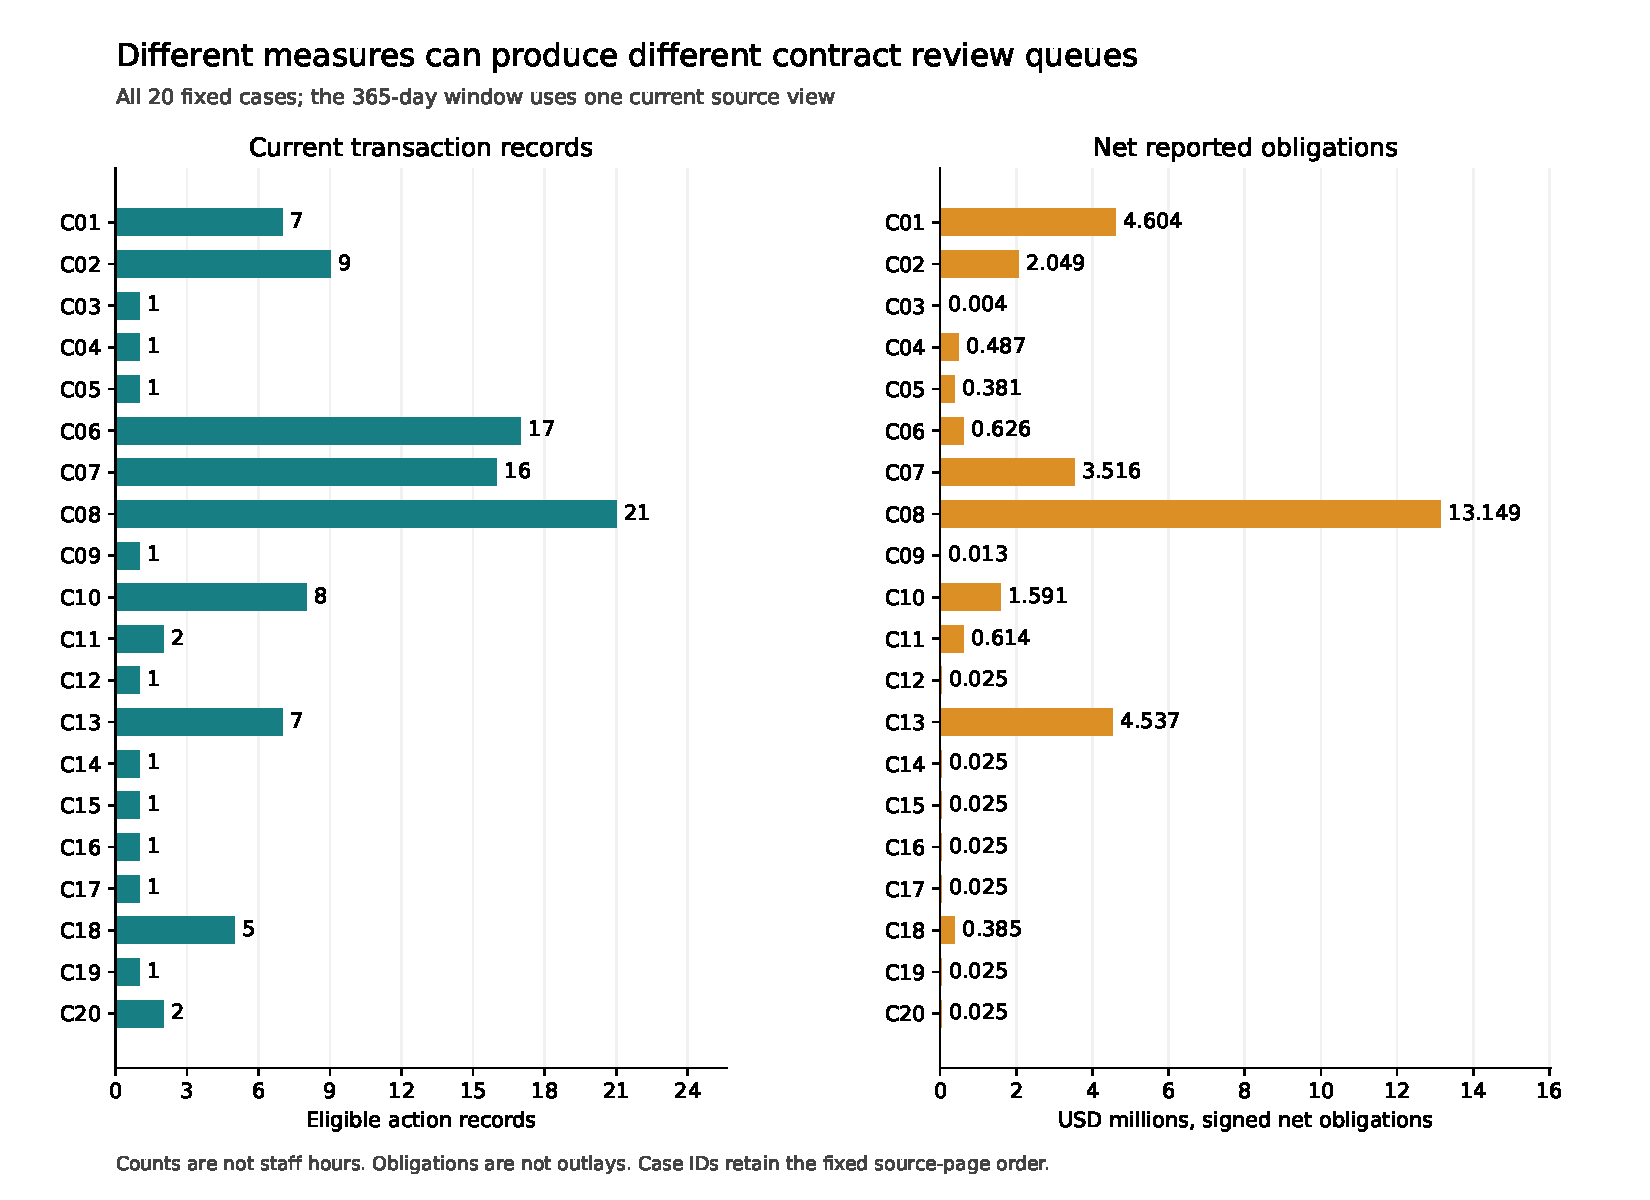
\includegraphics[width=9.45in,height=6.20in,keepaspectratio]{images/counts_and_obligations.pdf}\end{center}
\end{landscape}
\begin{landscape}
{\large\bfseries Signed financial offsets\par}
\vspace{3pt}
\begin{center}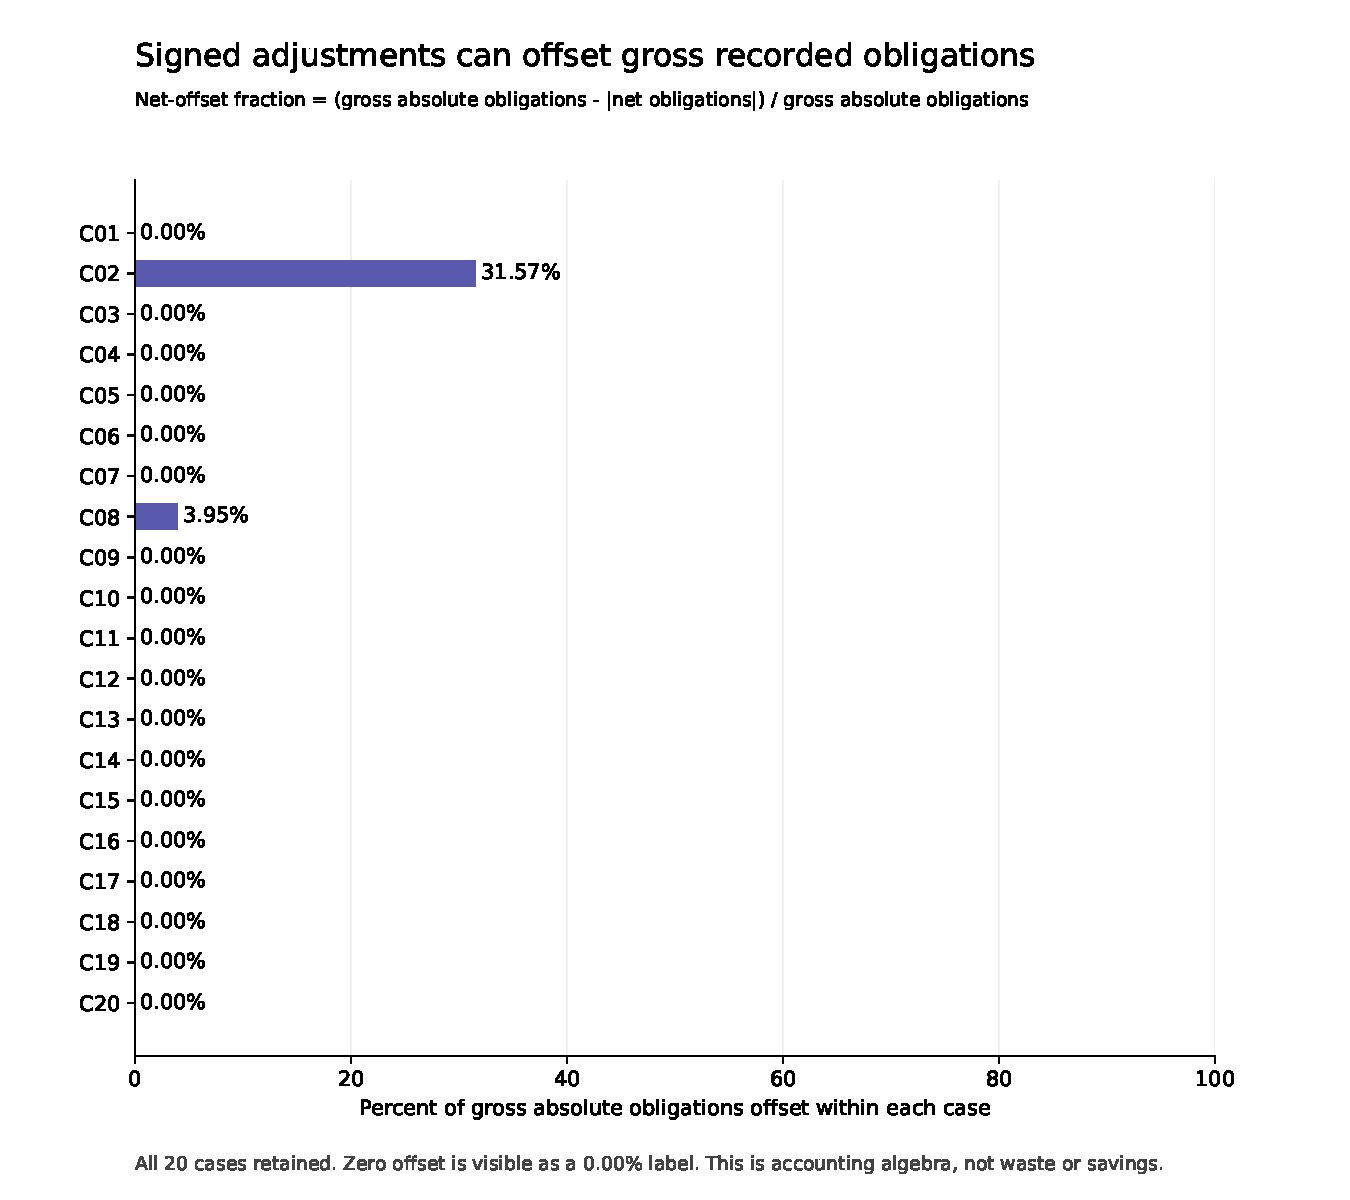
\includegraphics[width=9.45in,height=6.20in,keepaspectratio]{images/signed_offsets.pdf}\end{center}
\end{landscape}
\begin{landscape}
{\large\bfseries Fixed calendar-window probes\par}
\vspace{3pt}
\begin{center}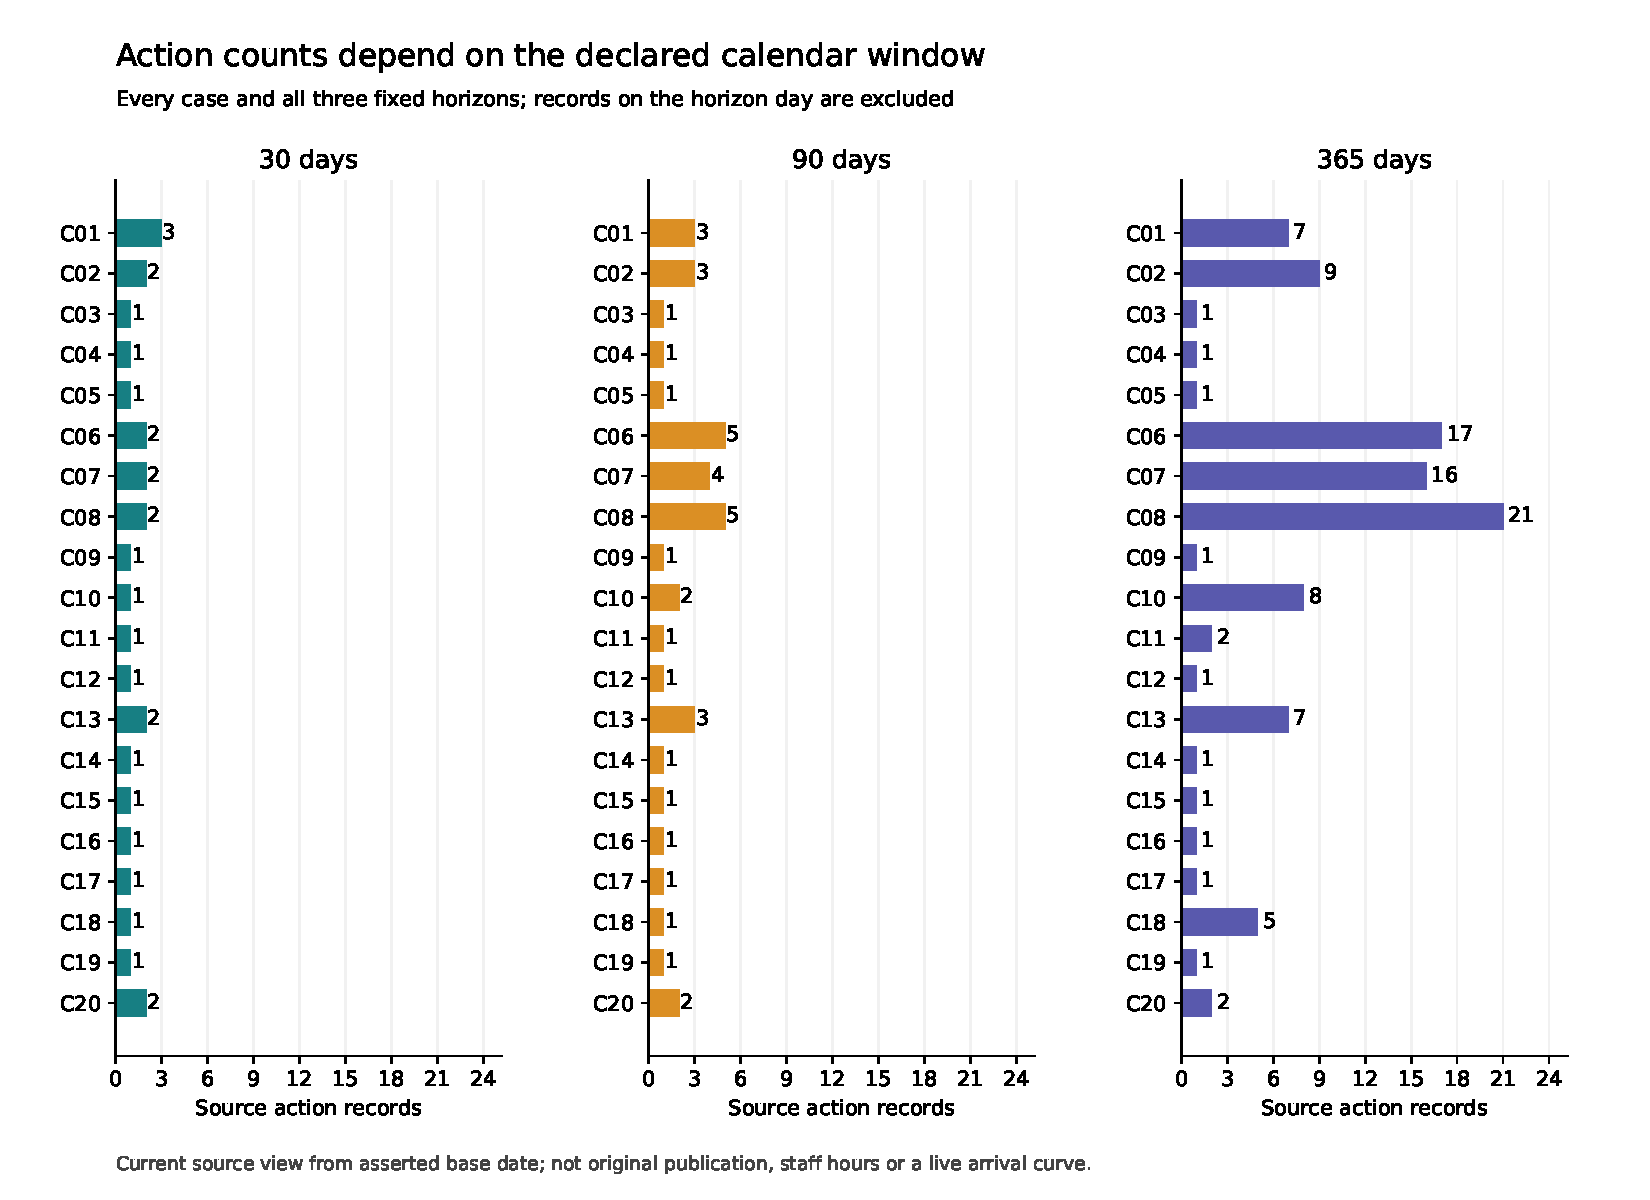
\includegraphics[width=9.45in,height=6.20in,keepaspectratio]{images/fixed_window_counts.pdf}\end{center}
\end{landscape}
\end{document}
